\section{Funktionsweise des flouriszierenden Aktinmarkers}
Für die Messung der Aktingeschwindigkeit wurde ein floursizierender Marker verwendet.
Floureszenz beschreibt eine spezielle Art der Abstrahlung von
Photonen durch einen quantenmechanischen Positionswechel
eines Elektron in einen energetisch niedrigeren Zustand.
Für Floureszenz brauch es ein Dreiniveausystem bei dem das
höchste Energieniveau kurzlebig, und das mittlere Energieniveau
sehr langlebig ist. Indem man die passende Lichtfrequenz verwendet,
regt Elektronen in das höchste Energieniveau an,
von dem sie sich schnell, ohne Photoemission, in das mittlere Niveau abregen.
In diesem Energieniveau verweilen sie, bis es spontan zu einer 
Abregung und der damit verbundenen Lichtemission kommt.
Da die Energiedifferenz zwischen mittlerem und niedrigstem Energieniveau kleiner ist als
die Energiediffernz zwischen dem niedrigsten und dem höchsten Niveau, ist die Wellenlänge
des Abgestrahlten Lichtes kleiner. Das wird schematisch in Abbildung
\ref{fig:dreiniveausystem} verdeutlicht.

\begin{figure}[]
  \centering
  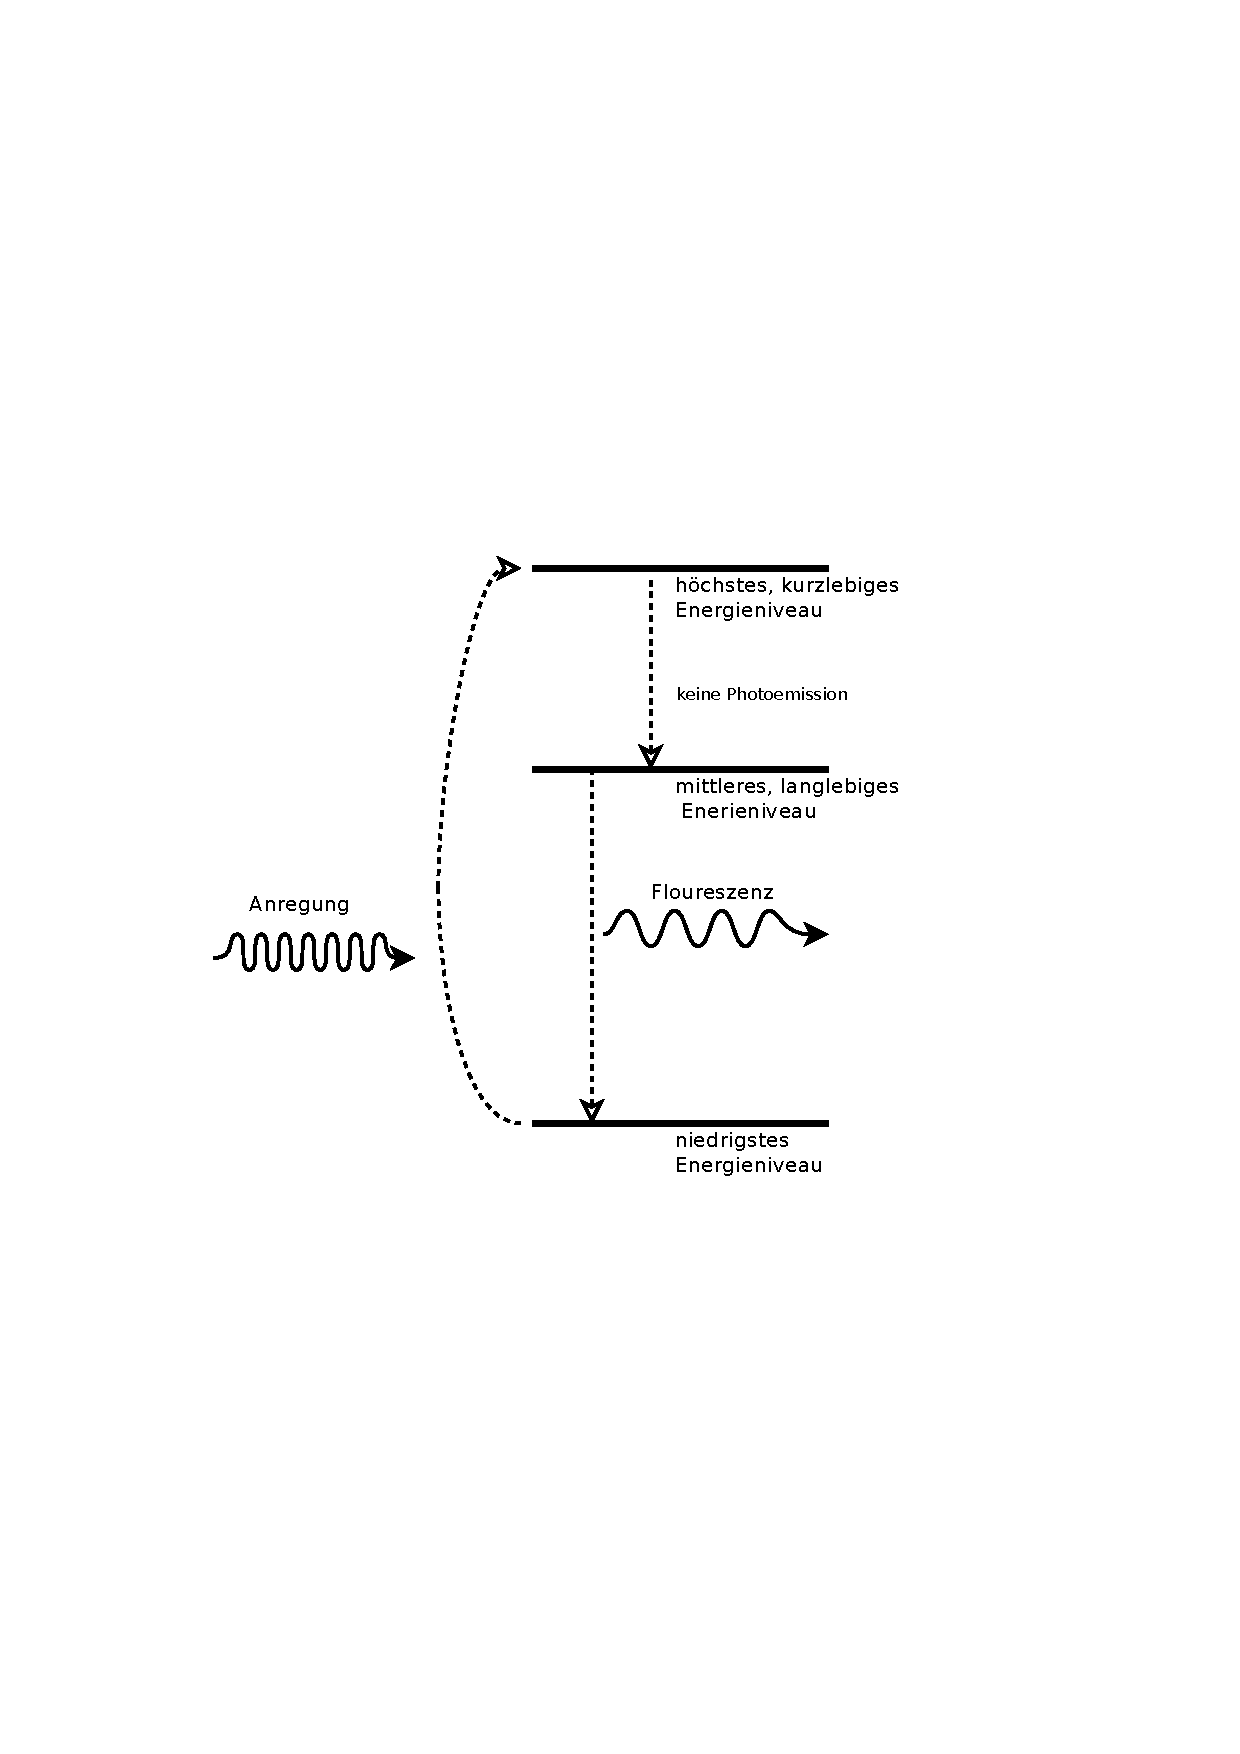
\includegraphics[width=\textwidth]{bilder/energieniveauschema.pdf}
  \caption{Ein Dreiniveausystem für Floureszenz}
  \label{fig:dreiniveausystem}
\end{figure}

\section{Zusammenhang zwischen numerischer Apertur und Auflösungsgrenze}
Um die Bewegung der Aktinfilamente in diesem Versuch zu beobachten, werden diese mit einem am Pilzgift Phalloidin gebundenen Farbstoff markiert.\\
Der hier zu beobachtende Effekt ist die Fluoreszenz. Atome fluoreszierender Stoffe werden durch Absorption von Photonen einer bestimmten Wellenlänge angeregt und beim Übergang in den Grundzustand wird ein Photon emittiert. In der Regel ist das emittierte Licht langwelliger als das eingestrahlte, dies lässt sich wie folgt erklären:\\
Bei der Anregung des Elektrons werden höhere Schwingungszustände des angeregten Zustands besetzt und ein Teil der Energie des anregenden Photons wird bei Schwingungsrelaxationen abgegeben. Zudem werden beim Zurückfallen des Elektrons in den Grundzustand auch zunächst höhere Schwingungszustände des Grundzustands besetzt. Diese Prozesse bedingen eine größere Wellenlänge des emittierten Lichts als die des absorbierten.\\
\\
Die Auflösung eines Objekts mithilfe eines Mikroskops wird zum einen von der Wellenlänge des bestrahlenden Lichts und zum anderen von der numerischen Apertur des benutzten Objektivs bestimmt. Strukturen, die kleiner sind als die verwendete Wellenlänge können nicht aufgelöst werden.\\
Die Auflösungsgrenze $d_{min}$ kann mit dem Rayleigh-Kriterium berechnet werden:
\begin{equation*}
d_{min}=\frac{1.22}{2}\cdot \frac{\lambda}{NA}
\label{eq:floureszenz}
\end{equation*}
\\
Als Fausregel merkt man sich $d_{min} \approx \frac{ \lambda}{N_{A}}$.\\
Hätten wir in unserem Versuch ein Auficht, oder ein Druchlichtmikroskop
für die Analyse der Aktingeschwindigkeit verwendet, hätten wir nach Gleichung \ref{eq:floureszenz} bei blauem
Licht mit $ \lambda = 488nm$ und der im Versuch gegebenen Linse eine
Auflösungsgrenze von 180 nm. \\
Die Auflösung des Floureszenzmikroskops beträgt $1.57 \sfrac{\mu m}{\text{Pixel}}$.
Bei einer Aktinlänge im Bereich von einigen $\mu m$ \cite{FOPRA_molecular_motors}
scheint die Auflösung eines gewöhnlichen Mikroskopes besser zu sein.
Jedoch würde man die Aktinstrukturen nicht erkennen, da es zu viel Streulicht gäbe.
So ist der Grund für die Verwendung eines Floureszenzmikroskopes der
deutlich bessere Kontrast des Floureszenzmikroskopes im Vergleich zum Auflicht-,
oder Durchlichtmikropskop.

%%% Local Variables:
%%% mode: latex
%%% TeX-master: "../motors"
%%% End:
